% report.tex
% Report.
% Copyright (C) 2010 Vladimir Rutsky <altsysrq@gmail.com>

% TODO: Use styles according to GOST (it's hard).

\documentclass[a4paper,10pt]{article}

% Encoding support.
\usepackage{ucs}
\usepackage[utf8x]{inputenc}
\usepackage[T2A]{fontenc}
\usepackage[russian]{babel}

\usepackage{amsmath, amsthm, amssymb}

% Indenting first paragraph.
\usepackage{indentfirst}

\usepackage{url}
\usepackage[unicode]{hyperref}

%\usepackage[final]{pdfpages}

\usepackage[pdftex]{graphicx}

\newcommand{\HRule}{\rule{\linewidth}{0.5mm}}

% Spaces after commas.
\frenchspacing
% Minimal carrying number of characters,
\righthyphenmin=2

% From K.V.Voroncov Latex in samples, 2005.
\textheight=24cm   % text height
\textwidth=16cm    % text width.
\oddsidemargin=0pt % left side indention
\topmargin=-1.5cm  % top side indention.
\parindent=24pt    % paragraph indent
\parskip=0pt       % distance between paragraphs.
\tolerance=2000
%\flushbottom       % page height aligning
%\hoffset=0cm
%\pagestyle{empty}  % without numeration

\begin{document}

% Title page.
% title.tex
% Report title page.
% Copyright (C) 2010 Vladimir Rutsky <altsysrq@gmail.com>

\begin{titlepage} % начало титульной страницы

\begin{center} % включить выравнивание по центру

\large Санкт-Петербургский государственный политехнический университет\\[4.5cm]
% название института, затем отступ 4,5см

\huge Отчет по лабораторной работе \No 1\\[0.6cm] % название работы, затем отступ 0,6см
\large по~курсу <<Компьютерная графика>>\\[1cm]
\large <<Представление криволинейной поверхности координатной сеткой 
с удалением невидимых линий методом плавающего горизонта>>\\[3.7cm]
% тема работы, затем отступ 3,7см

\begin{flushright} % выровнять её содержимое по левому краю
\begin{tabular}{l l}
\emph{Студент:} & Руцкий~В.\,В.\\
\emph{Группа:} & 4057/2\\
\emph{Преподаватель:} & Ильин~Ю.\,П.
\end{tabular}
\end{flushright} % конец выравнивания по левому краю

\vfill % заполнить всё доступное ниже пространство

{\large Санкт-Петербург 2010}
\end{center} % закончить выравнивание по центру
\thispagestyle{empty} % не нумеровать страницу
\end{titlepage} % конец титульной страницы


% Content


\section{Задание}
Требуется разработать программу, которая использует метод плавающего горизонта%
\footnote{\textit{Floating Horizon Algorithm}, описан в~%
\cite{rogers1989procelemsforcg, shikin1995cg, skala1985bresenhemmodif, ilyin2006task1}}
для удаления невидимых линий при визуализации криволинейной поверхности в классе непрерывных линий.

\subsection{Исходные данные}
Даны значения функции в узлах равномерной прямоугольной сетки:
$$ z_{ij} = F(x_i, y_j) $$
$$ x_i = x_0 + i \cdot \Delta_x \quad 0 \leqslant i \leqslant N $$
$$ y_j = y_0 + j \cdot \Delta_y \quad 0 \leqslant j \leqslant M $$

Задан видовой объём и размер поля вывода~\cite{ilyin2006task1}.

\subsection{Требуемый результат}
Необходимо получить проекцию заданной сеткой функции в соответствии с данными видовым объемом и полем вывода.
Невидимые линии должны быть удалены методом плавающего горизонта.

Должна быть предусмотрена возможность рисования линий одного направления: 
либо только линии вдоль оси $OX$ мировой системы координат, 
либо только линии вдоль оси $OY$.

\section{Детали реализации}
В соответствии с заданием был реализован алгоритм плавающего горизонта 
по описаниям из~\cite{rogers1989procelemsforcg, shikin1995cg, skala1985bresenhemmodif, ilyin2006task1}.

Видовой объем фиксирован прямоугольным параллелепипедом. 

Используется аксонометрическая проекция.

При отрисовке линий одного направления используется метод коррекции с помощью псевдорёбер.

\section{Интерфейс пользователя}
\begin{figure}[h!]
  \centering
  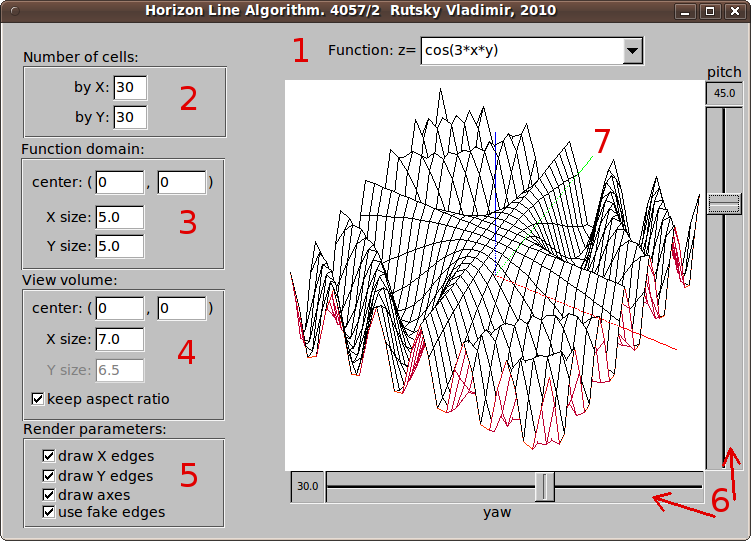
\includegraphics[width=0.8\linewidth]{./screenshots/ui_w-notes.png}
  \caption{Графический интерфейс пользователя}
  \label{fig:gui}
\end{figure}

Интерфейс пользователя приведён на рис.~\ref{fig:gui}.
Он состоит из следующих элементов:
\begin{enumerate}
  \item Выбор функции для отображения.
  \item Выбор размерности сетки.
  \item Выбор области определения функции. 
    Область задаётся своим центром и величинами половин ширины и высоты.
    Сетка $z_{ij}$ строится по области определения.
  \item Выбор размера видового объёма.
    Задаётся аналогично области определения.
    Опция <<Keep aspect ratio>> включает коррекцию выводимого изображения, 
    связанную с разными шагами по осям поля вывода.
  \item Параметры отрисовки:
    \begin{itemize}
      \item <<draw X/Y edges>>~--- выбор линий для рисования,
      \item <<draw axes>>~--- включение/выключение рисования осей координат
        (начало осей рисуется в центре видового объёма),
      \item <<use fake edges>>~--- включение/выключение использования псевдорёбер.
    \end{itemize}
  \item Задание преобразования поворота видового объёма.
    <<yaw>>~--- угол рыскания (в диапазоне $[-180^{\circ}, 180^{\circ}]$),
    <<pitch>>~--- угол тангажа (в диапазоне $[-90^{\circ}, 90^{\circ}]$).
  \item Поле вывода.
    Чёрным цветом рисуется верхняя часть поверхности, 
    розовым~--- нижняя. 
    Оси $OX$, $OY$ и $OZ$ рисуются красным, зелёным и синим соответственно.
\end{enumerate}

\section{Результат работы программы}
Результат работы программы представлен на рис.~\ref{fig:result1}, \ref{fig:result1-hor}, \ref{fig:result1-vert}.
\begin{figure}[h!]
  \centering
  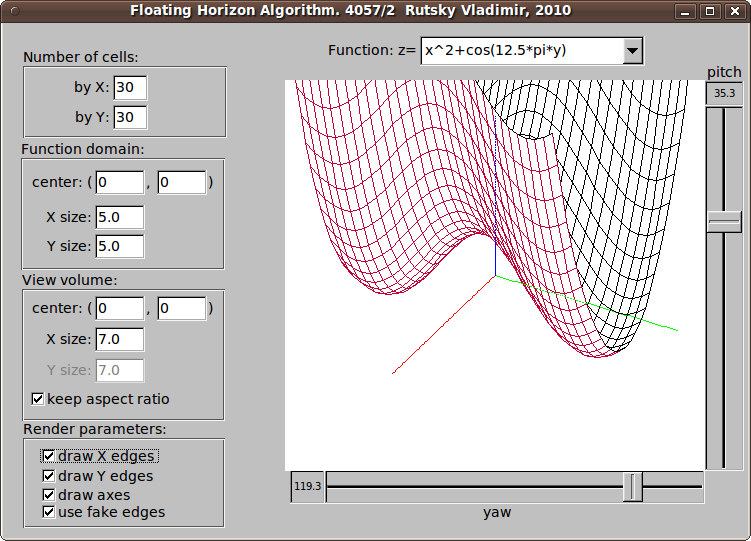
\includegraphics[width=0.8\linewidth]{./screenshots/result1.png}
  \caption{Результат работы программы. Общий случай}
  \label{fig:result1}
\end{figure}

\begin{figure}[h!]
  \centering
  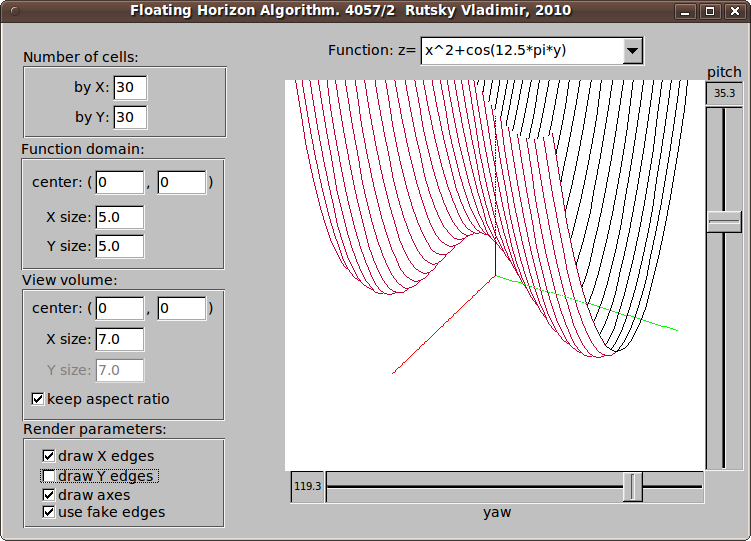
\includegraphics[width=0.8\linewidth]{./screenshots/result1_hor.png}
  \caption{Результат работы программы. Линии параллельные оси $OX$}
  \label{fig:result1-hor}
\end{figure}

\begin{figure}[h!]
  \centering
  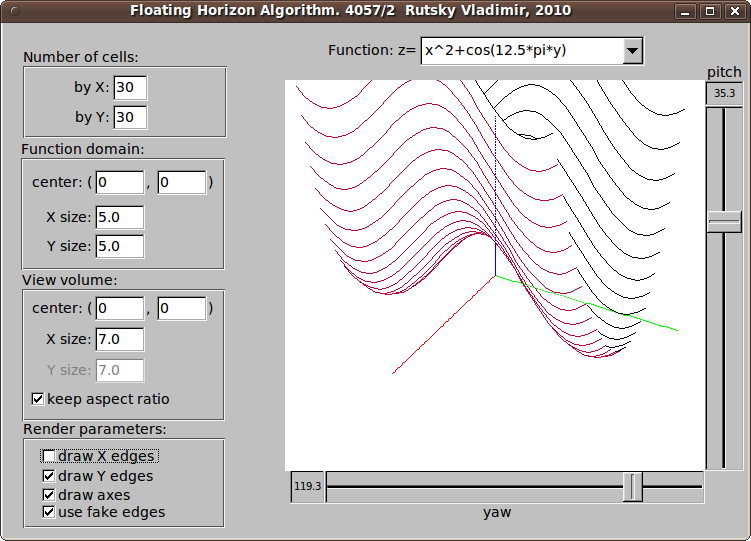
\includegraphics[width=0.8\linewidth]{./screenshots/result1_vert.png}
  \caption{Результат работы программы. Линии параллельные оси $OY$}
  \label{fig:result1-vert}
\end{figure}

\section{Среда разработки}
Программа разработана на языке С++ с использованием сторонних свободных кроссплатформенных библиотек.

Для сборки в среде GNU/Linux можно использовать средства \textit{GCC}%
\footnote{\textit{GNU Compiler Collection}, \url{http://gcc.gnu.org/}} 
(использовалась версия 4.4.1),
для сборки в среде Windows~--- Microsoft Visual Studio%
\footnote{\url{http://www.microsoft.com/visualstudio}}
(использовалась версия Microsoft Visual C++ 2008 Express Edition c SP1).

Графический интерфейс программы был реализован с использованием библиотеки \textit{FLTK}%
\footnote{\textit{Fast Light Toolkit}, \url{http://www.fltk.org/}}.

Работа с векторами, матрицами и афинными преобразованиями была реализована с использованием библиотеки \textit{Eigen}%
\footnote{\url{http://eigen.tuxfamily.org}}.

Для низкоуровневой работы с типами фиксированного размера была использована библиотека \textit{Boost}%
\footnote{\url{http://www.boost.org/}}.

\bibliographystyle{unsrt}
%\bibliographystyle{gost780u}
\bibliography{references.bib}

\end{document}
